In this chapter we define the multilevel regression model used throughout the rest of this thesis. We also set up and describe three data experiments that are the main contributions of this thesis. The primary goal of our model is to infer home advantage prior to and during the COVID-19 pandemic, thus we develop a model that has a home advantage parameter that we allow to vary across seasons whilst accounting for relative differences in teams offensive and defensive strengths. To motivate why the model is built the way it is we also conduct experiments to test the efficacy of multilevel regression modelling as well as the use of the Negative Binomial distribution opposed to the Poisson and Normal distributions more commonly used in regression analyses of sports data.

\section{Multilevel Model} \label{multilevel_model}

We infer home advantage by fitting a regression model to predict the points scored in each game while adjusting for relative team strengths and home advantage. We adjust for relative team strengths by modelling both an offensive rating and a defensive rating for each team. We argue this better represents real differences between teams and allows the model to better infer if a team performs better or worse when playing at home by measuring its performance relative to its average offensive performance versus its opponents average defensive performance. This section describes in detail the parameters of the model, their interpretation, and how we fit the model.

We aimed to build a parsimonious model to infer home advantage for each league while adjusting for relative team strengths and accounting for uncertainty in the data and parameter estimates. We needed a method that was robust to smaller sample sizes because we only had one COVID-19 adjusted season for each league to compare to and because this sample becomes smaller as you include more parameters, such as offensive and defensive team strengths for each team, which split the data into smaller groups from which we estimate the model parameters. We also wanted to be able to quantify the uncertainty in our parameter estimates. To address these concerns we adopt a Bayesian multi-level regression model framework building upon previous work \mbox{\cite{Baio2010} \cite{Glickman1998} \cite{Lopez2018} \cite{Benz2020}} that allows for pooling results across all teams to infer home advantage. The pooling occurs specifically for the parameters that represent offensive and defensive team ratings. The partial-pooling of multi-level regression modelling allows us to separate the effects of individual teams offensive and defensive strengths from their group level means while preventing over-fitting by adjusting parameter estimates through a process commonly referred to as ``shrinkage to the mean'' \mbox{\cite{Gelman2014} \cite{Gelman2006} \cite{McElreath2020}} as discussed in section \ref{Multilevel_Modelling}. We argue the pooling of data across each teams results to better handle smaller sample sizes while preventing over-fitting, and the ability to quantify the uncertainty in parameter estimates, makes Bayesian multi-level regression an ideal choice for this task.

We model the response variable of the number of points scored by each team in each game as Negative Binomial:

\begin{equation} \label{eq:likelihood}
y_{ij} | \mu_{ij}, \alpha_{ij} \sim \text{NegativeBinomial}(\mu_{ij}, \alpha_{ij})
\end{equation}

where \(y_{ij} = [y_{i1}, y_{i0}]\) is the vector of observed points scored in game \(i\) by the home (\(j=1\)) and away (\(j=0\)) teams and \(\mu_{ij} = [\mu_{i1}, \mu_{i0}]\) are the goal expectations of the home and away teams in game \(i\). The \(\alpha\) parameter allows for the flexibility of fitting to overdispersed data where the variance is much greater than the mean. In our experiments we have found that defining \(\alpha\) as a fraction of \(\mu_{ij}\) led to better sampling and model fit. Thus, we define \(\alpha_{ij} = \mu_{ij} * \lambda\) and then sample \(\lambda\) when fitting the model. We model the logarithm of goal expectation as a linear combination of explanatory variables:

\begin{equation} \label{eq:expected points}
\begin{split}
\text{log}(\mu_{i1}) &= \gamma_{sp} + \beta_{sp} + \omega_{sh[i]} + \delta_{sa[i]} \\
\text{log}(\mu_{i0}) &= \gamma_{sp} + \omega_{sa[i]} + \delta_{sh[i]}
\end{split}
\end{equation}

where \(\gamma_{sp}\) is the intercept term for expected log points in season, with \(s = [0, 1, 2, 3, 4]\) corresponding to the 2016, 2017, 2018, 2019, and 2020 seasons respectively. To instead model the situation where all previous seasons are combined and compared to the one COVID-19 adjusted season (see Figure \ref{fig:ha_pooled}), \(s\) is instead a binary indicator with \(s=0\) indicating all previous combined seasons and \(s=1\) indicating the COVID-19 adjusted season. The subscript \(p\) indicates regular season (\(p=0\)) or playoffs (\(p=1\)). Home advantage is represented by \(\beta_{sp}\) with \(s\) and \(p\) the same as the intercept. The offensive and defensive strength of the home and away teams are represented by \(\omega\) and \(\delta\). The nested indexes \(h[i]\) and \(a[i]\) identify the teams playing at home and away respectively and we use this nested notation to emphasize the multi-level nature of these parameters as they are modelled as exchangeable from a common distribution \cite{McElreath2020} \cite{Gelman2014} \cite{Gelman2006}. This enables pooling of information across games played by all teams in a league and results in mixing of the observable variables \((y_{ij})\) at this higher level which accounts for correlation in home and away points scored in each game \cite{Baio2010}. Note that the offensive and defensive strengths represented this way could potentially lead to problems of identifiability suggested by previous works \cite{Baio2010} \cite{Benz2020} \cite{Karlis2003} and fully described in \cite{McElreath2020}. The issue is that a given difference in relative team strengths can be solved by multiple different team ratings, similar to a system of equations being singular. In line with previous works \cite{Baio2010} \cite{Benz2020} \cite{Karlis2003}, we force the offensive and defensive ratings across all $T$ teams within each league to sum to zero for each season:

\begin{equation} \label{eq:sum to zero}
\sum_{t=1}^{T} \omega_{st} = 0, \sum_{t=1}^{T} \delta_{st} = 0
\end{equation}

Not only does this make identifiability a non-issue, but it also improves interpretability of the fitted team ratings as zero represents an average team rating with stronger and weaker ratings being correspondingly above or below zero. Also note that in this formulation defensive ratings are strong (weak) in the negative (positive) direction. This can be seen by considering how a negative defensive rating decreases the expected number of points in \ref{eq:expected points}, thus it represents a strong defensive team. Offensive ratings are the opposite by being strong (weak) in the positive (negative) direction.

In this model formulation we are estimating different home advantage parameters for the regular season and playoffs as well as for each individual season. The primary motivation for this is because the NHL and NBA COVID-19 bubbles essentially only occurred during their playoffs and we therefore want to separate home advantage during the playoffs for a more direct comparison. Modelling in this way also addresses potential questions of whether home advantage changes each year or remains constant. Our results in Figure \mbox{\ref{fig:ha_pooled}} are from estimating one home advantage parameter prior to COVID-19 and one afterwards. We then show the results of modelling home advantage separately for each season and show the results in Figure \mbox{\ref{fig:ha_main}} which reveal some interesting differences as discussed in the Results section.

In (\ref{eq:expected points}) we see that the home team's goal expectation is a linear combination of the home team's offensive strength and the away team's defensive strength as well as a constant home advantage. Conversely, the away team's goal expectation is a linear combination of the away team's offensive strength and the home team's defensive strength with the home advantage parameter noticeably missing. There is no index for league because we perform a separate model fit for each league. This is because each league varies greatly in their respective point totals which is explored further in the second experiment in section \ref{experiment_2}.

This model formulation results in the intercept representing the logarithm of the overall average of points scored with \(exp(\beta_{sp}), exp(\omega_{sh[i]}),\) and \(exp(\delta_{sa[i]})\) representing multiplicative increases or decreases to the average points scored to determine the expected points scored for an individual game. This can be seen by considering:

\begin{equation}
\begin{split}
\text{log}(\mu_{i1}) &= \gamma_{sp} + \beta_{sp} + \omega_{sh[i]} + \delta_{sa[i]} \\
\mu_{i1} &= \text{exp}(\gamma_{sp} + \beta_{sp} + \omega_{sh[i]} + \delta_{sa[i]}) \\
\mu_{i1} &= \text{exp}(\gamma_{sp})*\text{exp}(\beta_{sp})*\text{exp}(\omega_{sh[i]})*\text{exp}(\delta_{sa[i]})
\end{split}
\end{equation}

For example, a home advantage parameter of \(\beta = 0.25\) would result in multiplying the average points scored by \(\text{exp}(0.25) \approx 1.28,\) which can be interpreted as an increase of about 28\% in expected points scored by the home team in a game between teams with relative offensive and defensive strengths \(\omega_{sh[i]}\) and \(\delta_{sa[i]}\) respectively.

\subsection{Model Fit in PyMC3} \label{pymc3}

\begin{figure}
	\subfloat[]{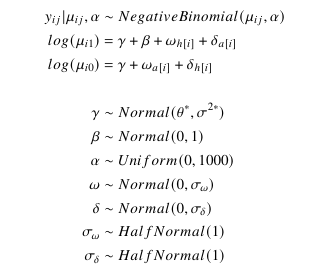
\includegraphics[width=0.28\textwidth]{figures/academic_model.png}} 
	\subfloat[]{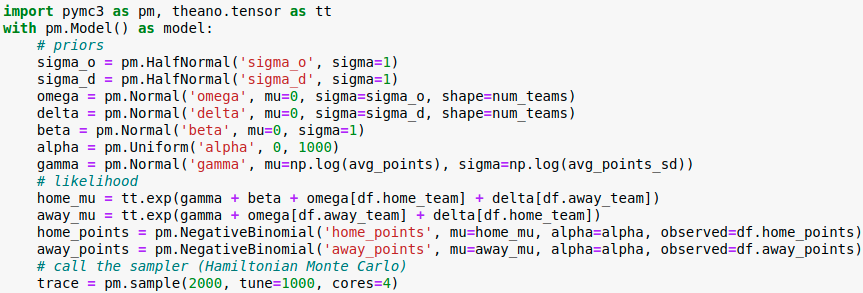
\includegraphics[width=0.72\textwidth]{figures/pymc3_code.png}}
	\caption{An example of how a Bayesian model would be defined in an academic textbook or paper (a) and how a probabilistic programming language such as PyMC3 would create the model in Python code (b). Note how the priors have to be defined first because the code will be executed procedurally. The two definitions are essentially identical otherwise.}
	\label{fig:pymc3_code}
\end{figure}

The models are fit using PyMC3, an open source probabilistic programming language (PPL) that allows us to fit Bayesian models with their implementation of a gradient based Hamiltonian Monte Carlo (HMC) No U-Turn Sampler (NUTS) \cite{pymc3}. PPLs are a tool for statistical modelling that try to bridge the gap between complex statistical definitions and easy to write code. They define a set of primitives for drawing random numbers and conditioning constructs. This enables defining random variables, how to sample them, storing their samples in memory, and how much weight to give them in a given execution of a program. For Bayesian modelling this means you can define all the variables in your model; whether they are priors, likelihoods, observed variables, or unobserved latent variables. Then you can sample all the variables in your model using any method supported by the PPL such as HMC. An example of how a model would be defined in an academic textbook or paper and then how it would be written in PyMC3 is shown in Figure \ref{fig:pymc3_code}. PPLs make defining and fitting models simpler and more accessible to non-experts. This allows for iteratively building and improving models as part of a workflow that would have been impossible for previous generations of scientists.

As in other previous work \cite{Baio2010} \cite{Benz2020}, we use Bayesian modelling and fitting approaches to allow us to incorporate some prior baseline knowledge of parameters as well as better quantifying uncertainty in the interpretation of parameter estimates. The Bayesian approach means we need to specify suitable prior distributions for all random parameters in the model. The prior distributions for parameters in our model are:

\begin{equation} \label{eq:priors}
\begin{split}
\gamma_{sp} &\sim \mathcal{N}(\theta^*, \sigma^{2*}) \\
\beta_{sp} &\sim \mathcal{N}(0, 1) \\
\lambda &\sim \text{Uniform}(0, 1000) \\
\omega_{st} &\sim \mathcal{N}(0, \sigma_{s\omega}) \\
\delta_{st} &\sim \mathcal{N}(0, \sigma_{s\delta}) \\
\sigma_{s\omega} &\sim \text{HalfNormal}(1) \\
\sigma_{s\delta} &\sim \text{HalfNormal}(1)
\end{split}
\end{equation}

where the offensive and defensive ratings for each team, \(\omega_{st}\) and \(\delta_{st}\) respectively for \(t=1,\dots,T\), are drawn from the same shared distributions, \(\mathcal{N}(0, \sigma_{s\omega})\) and \(\mathcal{N}(0, \sigma_{s\delta})\), which have their own priors, \(\sigma_{s\omega}\) and \(\sigma_{s\delta}\), known as hyperpriors. It is because each teams ratings are drawn from the respective same shared distribution that information is partially-pooled across teams while fitting the model. \(\theta^*\) is the logarithm of the average points scored, and \(\sigma^{2*}\) is the logarithm of the variance of points scored, over the regular seasons and playoffs of the league being modelled. We note that we found \(\gamma_{sp}\) fits close to \(\theta^*\) even when using a weakly informative prior, but we keep this formulation as it maintains the spirit of using prior information in Bayesian analysis. PyMC3's implementation of the Negative Binomial distribution defines the parameter \(\mu\) as the mean directly (a Poisson distribution parameter) and the parameter \(\alpha\) as a Gamma distribution parameter \cite{pymc3} such that the variance is equal to \(\mu\left(1 + \frac{\mu}{\alpha}\right)\). Thus the variance will generally be greater than the mean except for when \(\alpha \to \infty \). Since we have defined \(\alpha = \mu * \lambda\), the variance is then equal to \(\mu\left( 1 + \frac{1}{\lambda}\right)\). Therefore, we use a prior that allows \(\lambda\) to be small to model overdispersion while also allowing \(\lambda\) to potentially be large for instances where there is little to no overdispersion in the outcome variable and we instead want the Negative Binomial distribution to tend toward a Poisson distribution.

The model is fit using PyMC3's NUTS sampler using 4 chains of 2,000 iterations with 1,000 tune steps for a result of 8,000 samples from 12,000 total draws. It is standard practice to check convergence with the \(\hat{R}\) statistic from \cite{Gelman1992} \cite{Brooks1997}.  Each model fit produced \(\hat{R}\) statistics of 1.00 with no divergences \cite{Betancourt2017}, meaning the samples converged, the model fit is valid, and we can analyze the resulting parameter estimates to draw our inferences from.

\section{Experiments}

In this section we describe how the datasets we used were curated. We then set up and describe the three data experiments that make the main contributions of the thesis. The results are shown and discussed in the Results chapter.

\subsection{Data}

For each league we gathered data from the five most recent seasons spanning the years 2016-2020, both regular season and playoffs. For our model, for each game, we need to track the teams that are playing, which teams are home and away, their respective game point totals, which season the game occurred, and whether or not the game occurred in the playoffs or regular season.

The NHL data is sourced from Natural Stat Trick \cite{NS2020}. A typical NHL season consists of 82 games played by each team. Prior to the Vegas Golden Knights joining the league in 2017, there were 30 teams resulting in 1230 games per season. Since 2017 there are 1271 games played with 31 teams in the league. The playoffs consist of a bracket of 16 teams playing best-of-seven series, for an average of 80-90 games total. We note that the 2020 season was shortened to 1082 games due to stopping for the initial outbreak of the COVID-19 pandemic. The 2020 playoffs occurred inside the NHL bubble when play resumed, consisting of 6 games to determine positions 1-8 and 8 best-of-five series to determine positions 9-16 before beginning the usual playoff structure. This resulted in 129 games played in the NHL's COVID-19 bubble.

The NBA data is sourced from the basketball-reference website \cite{BR2020}. The structure of the regular season and playoff schedules is similar to that of the NHL. A typical NBA season consists of 30 teams each playing 82 games for a total of 1230 games. The playoffs consist of a bracket of 16 teams playing best-of-seven series, for an average of 80-90 games total. Like the NHL, the 2020 NBA season was shortened to 971 games due to stopping for the initial outbreak of the COVID-19 pandemic. The 2020 playoffs occurred inside the NBA bubble when play resumed, consisting of 8 additional games for each of the top 22 teams to determine seeding of the top 16 teams before beginning the usual playoff structure. This resulted in 172 games played in the NBA's COVID-19 bubble.

The MLB data is sourced from retrosheet \cite{RS2020}. A typical MLB season consists of 30 teams each playing 162 games for a total of 2430 games. The playoffs can be viewed as an 8 team bracket, but there are 4 ``wildcard'' teams that play two best-of-one games to determine the last two spots for the 8 teams that make the first round called the Division Series. The Division Series consists of best-of-five series to determine who moves on to the League Championship Series. The League Championship Series and the following World Series Championship consist of best-of-7 series to determine the winner. This playoff structure usually results in an average of 30-40 games. The 2020 COVID-19 restricted season reduced the number of scheduled games to 60 for each team. This change combined with cancellations due to outbreaks within teams reduced the total number of games to 898. The playoffs replaced the best-of-one wildcard round with best-of-three series involving all top 8 seeded teams. This resulted in a total of 52 playoff games. We note that the 2020 season saw some double-header games where teams switched home and away even though both games were played at the same stadium. We found this to have essentially no impact due these games making up a relatively small portion of total games (45/898) and to home advantage being so small in the MLB. We have reported the results with home and away defined as who batted last in each inning for all games.

The NFL data is sourced from the football-reference website \cite{FR2020}. A typical NFL season consists of 32 teams each playing 16 games for a total of 256 games. The playoffs usually consist of a bracket of the top 12 teams playing best-of-one games (the top 4 teams getting a first round ``bye'') resulting in 11 games total. Although the 2020 season had restrictions on fan attendance, the regular season schedule did not change and the playoff set-up only slightly changed by expanding to consist of the top 14 teams (only the top 2 getting a first round ``bye'') resulting in 13 games total. We exclude the Super Bowl as well as international site games from our analysis for consistency, as they are generally played at neutral sites and there are very few of them (i.e. 4-5 neutral site games out of a total 256 games each season).

\subsection{Complete pooling, No pooling, and Partial pooling} \label{experiment_1}

\subsubsection*{Objective}

In the Background on Bayesian Inference chapter we described the theory behind multilevel modelling and gave examples to motivate and explain why multilevel modelling is more effective than traditional regression modelling or simple averaging. For this experiment we want to explore how multilevel modelling performs on the datasets used in this thesis, as well as testing the efficacy of PSIS-LOO for estimating models out-of-sample predictive performance on sports data.

\subsubsection*{Models}

We create and compare three models in order to show the benefits of how multilevel modelling partially pools information across teams to improve model fit while preventing over-fitting. The first model is referred to as a \textit{completely pooled} model where the data from all teams is completely pooled into one overall average to be used. The completely pooled model adjusts the model described in section \ref{multilevel_model} by modifying equation \ref{eq:expected points} as follows:

\begin{equation} \label{eq:cp_model}
\begin{split}
\text{log}(\mu_{1}) &= \gamma_{sp} + \beta_{sp} \\
\text{log}(\mu_{0}) &= \gamma_{sp}
\end{split}
\end{equation}

This is the simplest regression model where an average number of points for home teams and away teams is calculated and then used for predictions.

The second model is referred to as a \textit{no pooling} model where essentially a separate regression fit is made for each team's offensive and defensive ratings; ignoring the information from other teams. This is a traditional regression model and is defined near identically to the model described in section \ref{multilevel_model}, with the only difference being that the team strength parameters are not pooled. In practice this means that the priors for the team strength parameters $\omega_s$ and $\delta_s$ described in equation \ref{eq:priors} are changed to $\mathcal{N}(0, 1)$. This prevents information being pooled across groups, hence the name no pooling.

Finally the multilevel model is fit as described in section \ref{multilevel_model}, which is referred to as a \textit{partially pooled} model for the context of this experiment. The effect of this model is shrinking the team strength estimates from the no pooling model towards the overall mean. This effect was described in section \ref{Multilevel_Modelling} and in theory helps to prevent over-fitting but worsening the fit to the training dataset in order to improve the out-of-sample fit. This experiment is designed to test how this theory holds up on the sports datasets considered in this thesis.

In the completely pooled model there is essentially one global average used for all groups and in this way the model has high bias and ignores the differences amongst groups. In the no pooling model each group has its own parameter fit, but completely ignores the data from other groups and how they are fit resulting in lower bias and a better fit to the data but at the risk of over-fitting. The partially pooled model is a balance between these two extremes allowing for a better model fit than the completely pooled model while better protecting against over-fitting than the no pooled model. The differences in team ratings from the no-pooled and partially-pooled models can be seen in the appendix.

\subsubsection*{Evaluation}

To compare these models we randomly split each sports dataset in half to create a train-set and test-set. The train-set is used to train each model and evaluate training fit, and then the model will also be evaluated on the test-set in order to approximate the fit on unseen data. Models are evaluated by computing their log-score as defined in \ref{eq:log-score}. We additionally compute the PSIS-LOO estimate for each model on the train-set to evaluate how well it approximates the log-score on the test-set. The same fitting and evaluating procedures are performed for each model on each dataset.

\begin{comment}
While one of the primary advantages of Bayesian models is computing a full distribution rather than only a point estimate, we can generate point estimates by taking the mean of the sample distribution of predictions for each model as their respective point estimate predictions to be compared to the actual data. The models are then compared by their mean squared error (MSE), with the results shown in Table ??. There are two key features that stand out in the results in Table ??. First, both the no pooling model and the partial pooling model have lower MSEs in both training and testing. This indicates that the completely pooled model is underfit and that the no pooling and partial pooling model do improve model fit by including group parameters (team ratings in this specific case). Second, the no pooling model provides the best model fit on the training data, but provides worse model fit than the partial pooling model on the test data. This shows the effect of regularization via shrinkage to the mean that was theoretical discussed earlier in section ??. These results give empirical evidence that multilevel models and their partial pooling provide improved model fit while protecting against overfitting, and is the reason we opted to use a multilevel model as the model of choice for inferring home advantage in this thesis.
\end{comment}

\subsection{Negative Binomial Regression} \label{experiment_2}

\subsubsection*{Objective}

Since point totals in sports are positive integers, the Poisson distribution is a natural choice for modelling their outcomes. The effectiveness of the Poisson distribution for modelling point totals has been shown in several works analysing European football data \cite{Karlis2003} \cite{Baio2010} \cite{Benz2020}. One shortcoming of the Poisson distribution is that it only has one parameter and this leads to the strong assumption that the mean is equal to the variance. For low scoring sports like European football and hockey, this is usually a fine assumption. However, this is an invalid assumption for several of the sports we analyse in this paper. Table \ref{tab:loo} reports the dispersion statistic \(\sigma_p\). The dispersion statistic represents how much greater the variance is than the mean while adjusting for sample size and model complexity. The dispersion statistics is computed as  \(\chi^2/(n-p)\) for each league, where \(\chi^2\) is the Pearson chi-squared statistic of the point totals data, and \(n-p\) are the degrees of freedom with \(n\) representing the sample size of the point totals data and \(p\) representing the number of predictors in our model. The commonly suggested threshold, \(\sigma_p > T\), for determining when a Poisson model is no longer appropriate is around \(1.2 < T < 2\) \cite{Payne2018} \cite{Cameron1990}. Table \ref{tab:loo} shows the NBA, MLB, and NFL having potential overdispersion in their point totals and thus, the Poisson distribution is likely inappropriate and less effective. This suggests the use of the Negative Binomial distribution because it has an extra parameter \(\alpha\) that gives greater flexibility and better model fit to data that is overdispersed while still adequately fitting models without overdispersion. This experiment is aimed at comparing and contrasting using the Negative Binomial distribution as the likelihood for our model opposed to the Poisson and Normal distributions that are more commonly used.

\subsubsection*{Models}

To establish the efficacy of the Negative Binomial distribution in our model, we fit and compare models using the Poisson and Normal distributions across each league. We fit Poisson and Normal regression models by changing the likelihood of the model in (\ref{eq:likelihood}) to \(y_{ij} | \mu_{ij} \sim \text{Pois}(\mu_{ij})\) for the Poisson regression (and subsequently drop \(\alpha\) from the rest of the model as it is not needed), and \(y_{ij} | \mu_{ij}, \sigma^2 \sim \mathcal{N}(\mu_{ij}, \sigma^2)\) for the Normal regression (and use a weakly informative prior \(\sigma^2 \sim \text{HalfNormal}(50)\)). Otherwise the models are identical and their interpretation remains the same as is discussed in the Methods section.

\subsubsection*{Evaluation}

We evaluate the models across each league by estimating the out-of-sample predictive fit via leave-one-out cross-validation (LOO). Following the work of Vehtari \cite{Vehtari2016} we approximate LOO using Pareto-smoothed importance sampling (PSIS) and report the results in Table \ref{tab:loo}. We note here that we also used the widely-applicable information criterion (WAIC) \cite{Watanabe2010} but found the results to be nearly identical and the conclusions the same.

\subsection{Inferring Home Advantage} \label{experiment_3}

\subsubsection*{Objective}

The primary goal of this thesis is to infer the potential effect of and change in home advantage in North American professional sports prior to and during COVID-19. After establishing the efficacy of our Negative Binomial multilevel regression model in the previous experiments, our final experiment is to fit our model to the datasets and then examine the distribution of the home advantage parameter and to discuss the implications.

\subsubsection*{Models}

To make inferences about home advantage prior to and during the COVID-19 pandemic we fit the multilevel model previously described in section \ref{multilevel_model}. The fitting of this model results in parameter estimated for home advantage across each of the four leagues analysed for four seasons prior to and one season during COVID-19.

\subsubsection*{Evaluation}

We examine the distributions of the parameter estimates for home advantage that result from the model fit. We analyse the trends and differences across seasons as well as leagues in order to make inferences and draw conclusions about the impact of home advantage in these sports.